\documentclass[12pt,oneside]{memoir}

\usepackage[biblatex]{matfmaster}
\usepackage{listings}

\bib{master}

\autor{Милош Самарџија}
\naslov{Развој микросервисне апликације за Android коришћењем окружења Lumen}
\godina{2020}

\mentor{др Милена \textsc{Вујошевић Јаничић}, доцент\\ Универзитет у Београду, Математички факултет}
\komisijaA{др Филип \textsc{Марић}, ванредни професор\\ Универзитет у Београду, Математички факултет}
\komisijaB{др Александар \textsc{Картељ}, доцент\\ Универзитет у Београду, Математички факултет}

% \datumodbrane{ }

% \apstr{ }

\kljucnereci{микросервиси, рачунарство, развојни оквир, андроид, трчање}

\begin{document}

\frontmatter
\naslovna
\komisija
\posveta{Мојој породици}
% \apstrakt
\tableofcontents*

\mainmatter

\chapter{Увод}
Микросервисна архитектура представљa један од популарнијих приступа развоју скалабилних дистрибуираних система. Главна филозофија на којој је овај приступ заснован је доменски оријентисано моделовање (енг. domain-driven design). Доменски оријентисано моделовање подстиче разбијање комплексних домена на што једноставније и независније поддомене, као и активно учешће доменских експерата (енг. domain experts) у развоју система.

Главна тематика којом се овај рад бави су основне идеје водиље доменски оријентисаног моделовања, на који начин их микросервисна архитектура инкорпорира, као и дизајн REST интерфејса за програмирање апликација (енг. RESTful API) који представљa једну од техника за интеграцију поддомена система. У те сврхе је осмишљенa и развијена апликација чији је циљ да илуструје примену микросервисне архитектуре у пракси, као и комуникацију са екстерним сервисима.

Апликација је названа MyRunningBuddy, а њена примарна намена је проналажење партнера за трчање на основу различитих параметара. Сам алгоритам за упаривање тркача уједно представљa и најважнији поддомен (енг. core subdomain) целог система који имплементира пословну логику и на који је потребно обратити највише пажњe током дизајна и имплементације. Део апликације је написан у програмском језику PHP коришћењем Lumen развојног оквира за развој микросервисних апликација и REST интерфејса за програмирање апликација, где је највећи део бизнис логике садржан. Други део апликације је написан у програмском језику Java, заједно са Android комплетом за развој софтвера (енг. Android SDK) и представља кориснички интерфејс, односно улазну тачку у систем, која није у фокусу овог рада, па ће према томе пропорционално мање времена бити утрошено за њен развој. У пракси, корисничка апликација и њен кориснички интерфејс су нешто на шта би подједнако требало обратити пажњу током развоја производа. За потребе складиштењa података од стране микросервиса користи се MySQL база података.
\chapter{Доменски оријентисано моделовање}
Доменски оријентисано моделовање је филозофија развоја чији циљ је управљање конструкцијом и одржавањем софтвера писаног за комплексне домене. Циљ се достиже употребом одређених образаца (енг. patterns), принципа и добрих пракси које, уколико се добро разумеју и примене, смањују шансу за прављење неких честих грешака које се јављају током развоја.
\section{Чести проблеми развоја пословних апликација}
Да бисмо разумели сврху постојања ове филозофије, потребно је да разумемо на какве изазове се најчешће наилази током развоја и одржавања софтвера. Један од популарнијих архитектуралних стилова коришћених у пословним апликацијама је тзв. велика лопта од блата (енг. Big Ball of Mud) коју карактерише лош дизајн кода са одсуством било какве организације. Такав софтвер је углавном доста спрегнут, и захтев за променом једне од функционалности може изазвати ланчану реакцију других измена које нису планиране, али су у том случају неопходне. Проблем је то што није лако уочљиво када пројекат скрене са правог пута, и од добре архитектуре дође до велике лопте од блата. Са временом се инкрементално квари, додавањем нових функционалности, и крпљењем постојећих, уз слабу бригу о одржању архитектуре, са изговором да ће некад касније бити издвојено време за рефакторисање. Тако настаје технички дуг (енг. technical debt).

Технички дуг је концепт у развоју софтвера настао као еквивалент новчаног дуга. Суштина концепта је да, занемаривањем дизајна кода, дуг постаје све већи, и све је мање вероватно да ће бити успешно измирен. У преводу, долази се до стадијума када је свака измена спецификације (која даље повлачи измене у коду) болна јер је софтвер постао изузетно спрегнут, и много компоненти зависи од других, иако у природи можда чак и не постоји таква веза између тих ентитета. Немогуће је направити изоловане измене, већ су оне раштркане широм система, и због тога се веома лако могу увести нови багови (енг. bugs) у систем. Јасно је да су измене спецификације у пословном софтверу неизбежне, па нам преостаје да се прилагодимо, или да пројекат полако али сигурно одведемо у пропаст. У тој ситуацији се, у зависности од тренутног стања кода, долази до закључка да је неопходно извршити опширно рефакторисање, или дизајнирање и писање софтвера испочетка. То све доводи до већих трошкова за развој, који су се могли избећи.
\section{Идеја филозофије и основни концепти}
Идеја водиља ове филозофије је разбијање великих и комплексних домена на једноставније поддомене. Ово има двојаки значај:
\begin{enumerate}
\item добијамо поддомене који су мање комплексни, и који имају јаснију одговорност
\item лакше се проналази и изолује најважнији поддомен у који је потребно уложити највећи део времена, јер је то оно што одређени софтвер чини другачијим од осталих решења, и представља разлог због којег је уопште и настао
\end{enumerate}

Такође, филозофија инсистира на томе да се у пројекат активно укључе и доменски експерти чија би примарна улога била упознавање програмера и остатка тима са комплексним доменом како би се избегле недоумице и погрешна решења. Ово функционише тако што се током целог развојног циклуса организују формални и неформални састанци са експертима, где се кроз дискусију и различите активности (енг. knowledge crunching) врши анализа и разбијање домена на више мањих, и моделовање поддомена. Као пропратни ефекат ових састанака настају аналитички модел, и заједнички језик (енг. ubiquitous language) чија је улога избегавање двосмислености у комуникацији између експерата и програмера. Током животног циклуса пројекта разумевање домена постаје боље, а заједно са разумевањем се развијају и расту заједнички језик и модели. Сва комуникација, модели и код су изражени у терминима заједничког језика.

\section{Аналитички модел}
Аналитички модел је колекција артефаката који описују модел система, и намена му је да програмерима и пословним корисницима помогне да боље разумеју домен. Да би овај модел имао смисла, све време мора бити усклађен са имплементационим моделом, тј. измене у имплементацији се морају огледати у изменама у аналитичком моделу, и обрнуто. Ова усклађеност постиже се управо изражавањем оба модела у терминима заједничког језика.

Да би се ово остварило, имплементациони модел мора да буде ослобођен било каквих брига које су техничке природе, и да буде фокусиран искључиво на домен. Такође, битно је да аналитички модел буде једноставан за имплементацију, тј. да не буде превише апстрактан, или на превише високом нивоу. Пројекти који постану тешки за одржавање управо пате од недостатка фокуса на домен; технички проблеми бивају помешани са доменском логиком, и дизајн кода се везује за техничке појмове, уместо за домен. То доводи до повећања сложености, и отежаног разумевања пројекта од стране нетехничких лица попут доменских експерата. Комуникација се успорава услед велике количине времена утрошеног на објашњавање техничких концепата нетехничким лицима, врло лако долази до неразумевања и јављају се двосмислености, а потом настају и погрешна софтверска решења.

\section{Врсте поддомена}
Разбијањем комплексног домена открива се више мањих и једноставнијих поддомена са мањим бројем одговорности. Сваки од поддомена се може сврстати у неку од категорија: главни, генерички (енг. generic) и потпорни (енг. supporting) поддомени. Уз сваки добијени поддомен се придружује његов одговарајући модел. Пример разбијања једног комплексног домена на више мањих може се видети на слици \ref{fig:razbijanjedomena}

\begin{figure}[!ht]
  \centering
  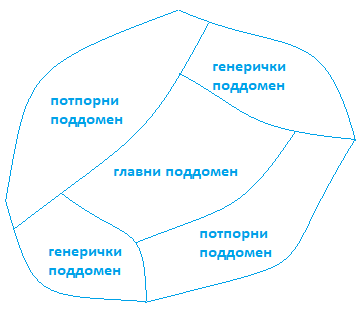
\includegraphics[scale=0.8]{slike/razbijanje-domena.png}
  \caption{Пример поделе комплексног домена на једноставније поддомене}
  \label{fig:razbijanjedomena}
\end{figure}

Под генеричким поддоменом се подразумевају неке од најраспрострањенијих функционалности које и већина других система такође има. Један пример генеричког поддомена може бити подсистем за слање и примање порука. Ово наравно не мора увек бити тачно. Генерички поддомен једног система може бити главни поддомен унутар другог система. У нашем примеру са подсистемом за поруке, у већини система ће вероватно бити сврстан као генерички, али ће представљати главни поддомен у системима чији је највећи адут управо размена порука.

У потпорни поддомен спадају све остале ствари које представљају подршку за функционисање главног домена. Заједничка ствар за потпорне и генеричке домене је то што су у односу на главни поддомен мање битни, али су неопходни јер без њих систем не може бити комплетан.

Главни поддомен садржи највећи и најбитнији део пословне логике, и у зависности од његовог модела и одговарајуће имплементације зависи да ли ће софтвер бити популаран и добро прихваћен, или ће се придружити великом броју других осредњих софтверских решења. Спецификација главног поддомена ће бити најподложнија изменама, и дизајнирању његовог модела треба приступити пажљиво, како би био довољно флексибилан да подржи све накнадне измене.

Са друге стране имамо потпорне и генеричке поддомене чији дизајн може бити слободнији, па се чак могу користити и неке готове софтверске библиотеке (енг. third party libraries). С обзиром да њихов модел не мора бити превише флексибилан, и највероватније ће трпети најмање измена, преживели бисмо и да се неки од њих временом претвори у велику лопту од блата. Кључно је то што је тај лош дизајн изолован од остатка система, и онемогућено му је даље ширење. Уместо претераног фокусирања на потпорне и генеричке поддомене, може се уложити додатни труд у развој главног поддомена. Програмери са мање искуства могу бити задужени за потпорне и генеричке поддомене, а они искуснији могу да се преусмере на главни поддомен.

\section{Доменски модел}
Доменски модел је централни појам доменски оријентисаног моделовања. На почетку се формира у виду аналитичког модела кроз заједничку сарадњу између развојног тима и доменских експерата. Не осликава домен у потпуности онако како изгледа у реалности, већ представља поглед на домен из једног угла, односно његову апстракцију, која је довољно добра за наше случајеве употребе. Слика \ref{fig:domenmodelprojekcija} приказује разлику између реалности и самог модела. Модел је описан заједничким језиком којим тим говори, као и дијаграмима које је тим креирао. Садржи само оно што је неопходно у контексту апликације која се креира, и мора да се развија паралелно са пословањем како би био користан и валидан. Модел је користан онолико колико је у стању да представи комплексну логику која решава пословне проблеме, а не колико добро осликава реалност.

Креирање доменског модела није једноставан посао, и представља итеративан процес. Велика је вероватноћа да први добијени модел неће бити задовољавајући, и то не треба да буде обесхрабрујуће. Тим би, заједно са доменским експертима, требало да настави са активностима, у циљу проналажења бољих модела. Не треба се задржати на само једном добром, већ треба пронаћи више задовољавајућих модела. Анализом доменских случајева употребе може се оценити корисност креираног модела, и потврдити да сви чланови тима разумеју домен.

Систем који се конструише се састоји од више целина, где су неке битније од других, па ће постојати више модела различите сложености које ће служити у различитим контекстима. С обзиром на захтевност овог процеса, комплексни и богати модели се креирају само за битне поддомене система. 

\begin{figure}[!ht]
  \centering
  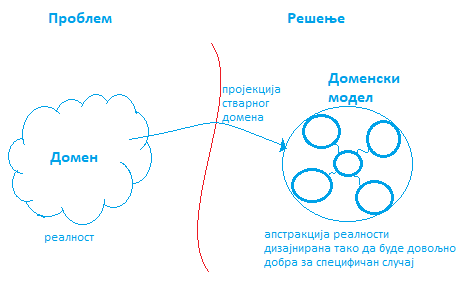
\includegraphics[scale=0.8]{slike/domen-model-projekcija.png}
  \caption{Пројекција реалног домена на једну његову апстракцију}
  \label{fig:domenmodelprojekcija}
\end{figure}
\subsection{Имплементациони обрасци за доменски модел}
Уколико посматрамо слојевите архитектуре софтвера, слој домена би представљао срж апликације. Он изолује сложеност доменског модела од сложености разних техничких делова софтвера. Његова улога је да осигура да се техничке ствари попут логике за управљање трансакцијама, складиштења података и приказивања не умешају у комплексност пословне логике. Мешањем инфраструктурне и пословне логике добили бисмо код који је тежи за разумевање, јер има више од једног задужења, и не можемо се фокусирати на само једну ствар. Слој домена обично представља само мали део целокупне апликације, што се може видети на слици \ref{fig:slojevitaarhitektura}.

\begin{figure}[!ht]
  \centering
  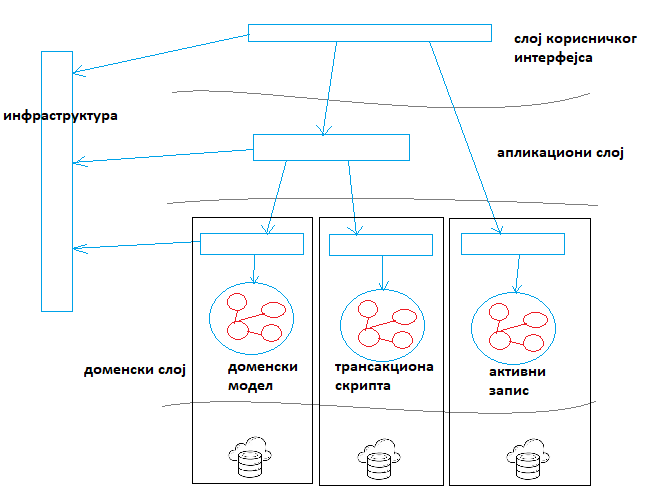
\includegraphics[scale=0.8]{slike/slojevita-arhitektura.png}
  \caption{Слој домена као део сложеније архитектуре}
  \label{fig:slojevitaarhitektura}
\end{figure}

Конструкција доменских модела је проблем који нема јединствено решење, али у пракси постоје одређена решења, односно имплементациони обрасци, који су општеприхваћени и углавном су се добро показали. Неки од њих више одговарају сложенијим поддоменима, док се други могу искористити код једноставнијих, за прављење простијих и сиромашнијих модела. Популарнији обрасци који се користе су доменски модел (енг. domain model), трансакциона скрипта (енг. transaction script) и активни запис (енг. active record).

\subsubsection{Образац "доменски модел"}
Овај образац се најбоље уклапа у комплексне домене са богатом пословном логиком, и подразумева креирање објектно-оријентисаног модела који садржи податке, пословне процесе и правила, и богату доменску логику. Премиса обрасца је да не постоји база података, и да током еволуирања модела проблем складиштења података буде занемарен. Објекти у добијеном моделу су у потпуности ослобођени од инфраструктурних проблема, што нам омогућава да дизајн нашег модела буде фокусиран искључиво на домен. На слици \ref{fig:razdvajanjedomenskogsloja} се може видети како је доменски слој раздвојен од техничких ствари попут складиштења података.

\begin{figure}[!ht]
  \centering
  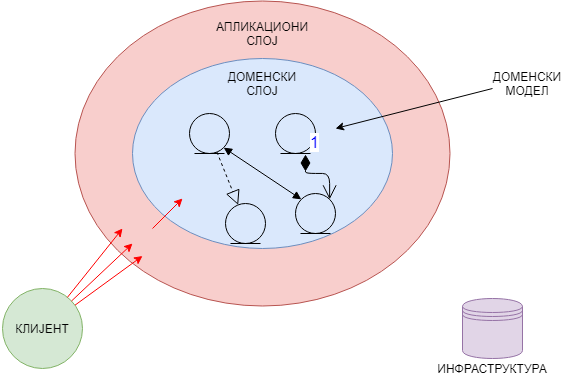
\includegraphics[scale=0.8]{slike/razdvajanje-domenskog-sloja.png}
  \caption{Раздвајање доменског слоја од остатка апликације}
  \label{fig:razdvajanjedomenskogsloja}
\end{figure}

\subsubsection{Образац "трансакциона скрипта"}
Трансакциона скрипта је, за разлику од доменског модела, заснована на процедуралном стилу развоја, лакша је за разумевање и имплементацију. Идеја је да се за сваки пословни случај употребе креира по једна процедура, и да се све те процедуре групишу на једно место. Свака од процедура треба да садржи сву логику потребну да се обави одговарајући случај употребе, укључујући ствари попут пословних правила, логике за складиштење података, итд. Предност овог обрасца су једноставност и могућност да се лако имплементирају нови случајеви употребе додавањем нове процедуре, без бојазни да ли ће бити утицаја на постојећу функционалност. Мане су, очигледно, потенцијално много понављања исте логике на различитим местима и лоша подела одговорности. Овакав образац је најприхватљивији за једноставније поддомене који садрже мало логике.

\subsubsection{Образац "активни запис"}
Активни запис је популарни образац који подразумева да се сваки објекат модела пресликава у одговарајући ред неке табеле. Погодан је у случајевима када модел базе података одговара пословном моделу. Ова структура ће у себи садржати податке и понашање, као и додатне методе за складиштење, додавање нових инстанци и претраживање колекције објеката. С обзиром да свака од структура има методе за креирање, читање, ажурирање и брисање, могуће је коришћење алата и скриптова за аутоматско генерисање доменског модела.

\chapter{Закључак}

\literatura

% \backmatter

\end{document} 
